\documentclass[a4paper, twoside, 12pt]{scrreprt}
%\documentclass[headsepline,titlepage,twoside,12pt]{report}
\linespread{1.25}
\usepackage[ngerman]{babel}
\usepackage[T1]{fontenc}
\usepackage[utf8]{inputenc}
\usepackage[a4paper,top=4cm,bottom=3cm,left=4cm,right=3cm]{geometry}
\usepackage{amsmath}
\usepackage{amssymb}
\usepackage{color}
\usepackage{graphicx}
\usepackage{soul}
%\usepackage{natbib}
\usepackage{hyperref}
\usepackage{listings}
\usepackage{textcomp}
\usepackage{microtype}
\usepackage{tabularx}
\usepackage{setspace}
\usepackage{booktabs}
\usepackage[locale=DE]{siunitx}
%\sisetup{output-decimal-marker = {,}}
\sisetup{decimalsymbol=comma}
\usepackage{todonotes}% Für Anmerkungen
\presetkeys{todonotes}{inline,backgroundcolor=yellow}{}
\usepackage{csquotes}
\MakeOuterQuote{"}
\lstset{frame=tb,
  language=HTML,
  aboveskip=3mm,
  belowskip=3mm,
  showstringspaces=false,
  columns=flexible,
  basicstyle={\small\ttfamily},
  numbers=none,
  numberstyle=\tiny\color{gray},
  keywordstyle=\color{blue},
  commentstyle=\color{teal},
  stringstyle=\color{red},
  breaklines=true,
  breakatwhitespace=true,
  tabsize=3,
  texcl=true,
}

\lstset{
  literate={ö}{{ö}}1
           {ä}{{ä}}1
           {ü}{{ü}}1
}
\title{Besondere Lernleistung}
\author{Gernot Zacharias}
\subtitle{Webanwendung zum Finden eines optimalen Standortes durch Distanzminimierung mithilfe von Online-Kartendiensten}
\begin{document}
%\listoftodos
\maketitle
\cleardoublepage
\tableofcontents
%\chapter* {Inhaltsverzeichnis}
\setcounter{page}{1}
\chapter*{Zusammenfassung}
\addcontentsline{toc}{chapter}{Zusammenfassung}
Durch den aufstrebenden Online-Versandhandel, wie zum Beispiel durch Online-Versandapotheken, entstehen neue Probleme.
Die Versandhändler benötigen Lagerhäuser für ihre Waren und die Fahrtwege vom Lager zum Kunden sollten möglichst minimal gehalten werden, um Zeit und Geld zu sparen.
Durch die Verkürzung der Fahrwege wird auch die Gesundheit und die Natur weniger belastet.
Auch Privatanwender profitieren von kurzen Fahrtwegen.
Dieses Problem lässt sich durch eine Anwendung lösen, die aus der Häufigkeit der angesteuerten Orte eine optimale Position mit möglichst kurzen Fahrwegen bestimmt.
Diese Anwendung kann zum Beispiel auf Basis der Kartendienste von "Google Maps" oder "Open Street Map" realisiert werden.
Dies lies sich am einfachsten durch eine Webanwendung lösen, da diese meistens plattformunabhängig sind.
Somit ist keine Installation von zusätzlicher Software, außer einem aktuellen Webbrowser, nötig.
Des weiteren habe ich mich für den freien Kartendienst von \emph{Open Street Map} entschieden, da dieser die meiste Freiheit bietet.
Auch gibt es für Open Street Map eine größere Auswahl an Nutzerschnittstellen.
Die Anwendung funktioniert sehr gut.%\todo{Fragebogen}
Somit lässt sich auch der Treibstoffverbrauch reduzieren, was dem Geldbeutel und der Umwelt zu Gute kommt.
Es gab auch positives Feedback von anderen Personen, die das Programm getestet haben.
Allerdings bietet die Anwendung auch noch viel Spielraum für individuelle Erweiterungen, Verbesserungen und Änderungen.
\chapter*{Abkürzungsverzeichnis}
\addcontentsline{toc}{chapter}{Abkürzungsverzeichnis}
\begin{tabularx}{\textwidth}{lX}
\toprule
\textrm{Begriff}                &\textrm{Erklärung des Begriffs}\\
\midrule
API		&Application Programming Interface\\
CSS		&Cascading Style Sheets\\
GIS		&Geographic Information System \\
HTML	&Hypertext Markup Language\\
HTTP	&Hypertext Transfer Protocol\\
HTTPS	&Hypertext Transfer Protocol Secure\\
JS		&JavaScript\\
PNG		&Portable Network Graphic\\
%WGS84	&52\\
WWW		&World Wide Web\\

\bottomrule
\end{tabularx}

\chapter{Einleitung}
\section{Gegenstand und Motivation}
\subsection{Gegenstand}
%\todo{Verdoppelung von "sich einen möglichst kurzen Weg". Stört mich nicht aber eventuell den Deutschlehrer.}
%\todo{Ich bin immer vorsichtig mit "viele X" und "immer mehr X" wenn man dazu keine Belege hat.}
\begin{itemize}
\item Viele Versandhändler suchen sich einen möglichst kurzen Weg zum Kunden oder zur Produktionsstätte.
\item Normalverbraucher wünschen sich einen möglichst kurzen Weg zu ihrer Arbeit, zum Kindergarten, Arzt, $\ldots{}$
\end{itemize}
\subsection{Problematik}
\begin{itemize}
\item Durch lange Fahrtwege erhöht sich die Dauer der Fahrt bis zum Ziel und somit der Energieverbrauch sowie die Schadstoffbelastung.
\item Auch die Kosten erhöhen sich bei langen Fahrten, da der Fahrer und/oder der Treibstoff bezahlt werden muss.
\end{itemize}
\section{Motivation}
\begin{itemize}
\item Durch die Reduktion der Distanz zum Ziel wird der Energieverbrauch und die Zeit verringert.
\item Aufgrund der Reduktion der Fahrtwege wird Geld gespart und die Umwelt geschont.
\end{itemize}
\section{Problemstellung}
Der Online Versandhandel ist ein zurzeit stark wachsender Sektor der Wirtschaft.\cite{Stepper2016}
Deshalb verwundert es auch nicht das es heutzutage
Es gibt auch Online-Versandapotheken, welche Medikamente an die Haustür liefern.
Dies ist vor allem für bewegungseingeschränkte Personen interessant, da diese sich nun nicht mehr zu nächsten Apotheke bewegen müssen.
Auch ermöglicht es Personen die nicht in der Nähe einer Apotheke wohnen, sich die benötigten Medikamente zu besorgen.
Für die Anbieter dieser Versandapotheken ist es nun interessant herauszufinden, wie man Zeit und Geld beim Versand einsparen kann.
Dazu kann man zum Beispiel die Warenlager dort plazieren, wo die Nachfrage am größten ist.
\section{Zielsetzung}
Das Ziel ist es eine Anwendung zu kreieren, welche aus der Häufigkeit des Ansteuerns von bestimmten Orten, einen Ort bestimmt, von welchem aus die Gesamtdistanz,in Abhängigkeit von der Häufigkeit, zu den gegebenen Orten, möglichst klein ist.
\section{Aufgabenstellung}
Zur Lösung der oben genannten Probleme soll eine Webanwendung erstellt werden, welche eine Karte anzeigt, auf der der Nutzer/-in Standorte auswählt, die er mit einer bestimmten Häufigkeit, die er/sie/es selbst angibt, aufsucht.
%\section{Aufbau der Arbeit}
\section{Existierende Lösungen}
Die WIGeoGIS\footnote{\url{https://www.wigeogis.com} [02.04.2019 10:58]} Softwareerstellungs- und Handelsgesellschaft m.b.H. bietet verschiedene Services für Kunden aus dem Industriesektor an, unter anderem WebGIS zur Datenanalyse, die über verschiedene Schnittstellen eingebunden werden können, auf digitalen Landkarten. 
Auch bieten sie eine kostenpflichtige Erweiterung des OpenSource Programms QGIS an, um Kunden Daten zur Marktlage oder Bevölkerung zur Verfügung zu stellen.
Das als Opensource verfügbare Programm QGIS ist für Laien recht unübersichtlich und überfordert durch zu großen Funktionsumfang. Bei der Anwendung handelt es sich auch nicht um eine Webanwendung, wodurch der Nutzer zusätzlich Software herunterladen muss.

\chapter{Grundlagen}
\section{World Wide Web}
In der heutigen Zeit gewinnt das World Wide Web (WWW) immer mehr an Bedeutung und ist fast schon nicht mehr wegzudenken.
Das World Wide Web ist der Teil des Internets, in dem die Daten mithilfe des HTTP/HTTPS -Protokolls ausgetauscht werden, wobei ein Computer, der Server mit der entsprechenden Webseite, die Daten auf Anfrage des Clients zu diesem schickt.
Das WWW umfasst also fast alle öffentlich zugänglichen Webseiten.
\section{HTML}
Die Hyper Text Markup Language (HTML) ist die benutzte Sprache im WWW und beschreibt eine Textdatei, in welcher mit einer bestimmten Syntax geschrieben werden muss.
Diese Textdatei wird dann von einem Browser analysiert und zeigt dem Endnutzer den Text mit entsprechender Formatierung.
Reine HTML Webseiten besitzten keine dynamischen Elemente und bieten dem Nutzer wenig Interaktionsmöglichkeiten.
\section{JavaScript}
JavaScript ist eine Scriptsprache welche direkt in eine HTML Datei implementiert werden kann und auch vom Browser entsprechend verarbeitet wird und dynamische Webseiten erlaubt.
JavaScript wird über das \verb+<script>...</script>+ -tag in die HTML Datei eingebunden.
%\section{Geographische Koordinaten}
%Geographische Koordinaten werden in Längen- und Breitengrad angegeben. 
%\section{Kartenprojektion}
%Die Karte von OpenStreetMap nutzt die Merkatorprojektion
\section{Google Maps}
Google Maps\footnote{\url{https://www.google.com/maps/} [18.06.2019 11:18]} ist der bekannste Online Kartendienst und bietet viele Möglickeiten zum erstellen von dynamischen Kartendarstellungen auf der eigenen Webseite.
Allerdings benötigt man zur Nutzung der Google Maps API\footnote{\url{https://cloud.google.com/maps-platform/} [18.06.2019 15:42} einen benutzerbezogenen Key, welchen man allerdings nur gegen Angabe von Kreditkarten Informationen erstellen kann.
\section{Open Street Maps}
Open Street Maps\footnote{\url{https://www.openstreetmap.org/about}  [02.04.2019 11:01]} spielt im Vergleich mit Google Maps eine untergeordnete Rolle.
Dafür bietet Open Street Maps freies Kartenmaterial an und es steht eine große Menge an freien APIs.
In meinem Prototypen setze ich auf Leafelet\footnote{\url{https://leafletjs.com/} [18.06.2019 15:07]}, welches die Kartendaten über eine externe Webseite bezieht, welche das Kartenmaterial von Open Street Maps als .png zur Verfügung stellt.
%\section{Gegenüberstellung von Google Maps und Open Street Maps}

\chapter{Algorithmus}
Um den Mittelpunkt der Längen- und Breitengrade zu berechnen nutzte ich folgenende Gleichung zur Berechnung von Längengrad und Breitengrad:
\begin{eqnarray}
\displaystyle
\lambda = \left(\sum_{i=1}^{n}\lambda_i \cdot w_i \right) \cdot \left(\sum_{i=1}^{n} w_i \right)^{-1}\\
\varphi = \left(\sum_{i=1}^{n}\varphi_i \cdot w_i \right) \cdot \left(\sum_{i=1}^{n} w_i \right)^{-1}
\end{eqnarray}
Die Anwendung berechnet einen gewichteten Mittelpunkt anhand der vom Nutzer angegebenen Priorität.
Wärend des Setzens der Marker wird bereits ein Mittelpunkt berechnet.
Durch einen Klick auf den Marker erscheint ein Popup in welchem man die Priorität ändern kann. 
Danach wird die Position des Mittelpunktes erneut berechnet.
Der Mittelpunkt wird durch drei Kreise dargestellt, einen inneren roten, einen mittleren gelben und durch einen grünen äußeren Kreis.
\chapter{Implementierung}
Für die Kartendarstellung wird Leaflet\cite{crickard2014leaflet}, eine OpenSource Bibliothek für die Darstellung von Kartenmaterial aus verschiedenen Quellen, genutzt. Eine Kartendatenquelle, die diese Anwendung benutzt, ist OpenStreetMaps.
Für die Webanwendung ist nur ein halbwegs aktueller Webbrowser notwendig, welcher in der Lage ist, Javascript Anwendungen ausführen zu können.
Die Webanwendung besteht im wesentlichen bloß aus einem HTML Dokument und einer Javascript Datei sowie der Leaflet Bibliothek.
\begin{lstlisting}
	...
	<link rel="stylesheet" href="leaflet/leaflet.css" crossorigin=""/>
	<script src="leaflet/leaflet.js"></script>
	...
	<div id="map"></div>
	<script src="js/leafscript1.js" type = "text/javascript"></script>
	...
\end{lstlisting}
Das Script \textit{leaflet1.js} erstellt eine neue Variable \textit{mymap}, die dann als Objekt für die Kartendaten dient.
Die Karte wird dabei erstellt und hat als Mittelpunkt die Stadt Leipzig (Längengrad: \si{51{,}339}{\textdegree}  Nord, Breitengrad: \si{12{,}381}{\textdegree}  Ost). Die Ansicht ist standardmäßig auf eine Zoomstufe von 12 eingestellt, da man so die gesamte Stadt und das Umland sehen kann.
Als nächstes wird dann zur Karte eine neue Ebene hinzugefügt, welche die Bildinformationen von einem OpenStreetMap Server abfragt und darstellt.
Außerdem wird festgelegt wie weit man in die Karte hinein- und hinauszoomen kann.
\lstset{language=Java}
\begin{lstlisting}
const mymap = L.map('map').setView([51.33918, 12.38105], 12);
L.tileLayer('http://{s}.tile.osm.org/{z}/{x}/{y}.png?lang=de', {
	maxZoom: 20,
	minZoom: 5,
	attribution: '&copy; <a href="http://osm.org/copyright">OpenStreetMap</a> contributors',
}).addTo(mymap);
\end{lstlisting}
Als nächstes wird eine Varible für einen Marker initialisiert, sowie eine Konstante i und ein Feld für die gesetzten Marker. Auch werden Variablen für die Kreise, die den Mittelpunkt anzeigen, definiert.
\begin{lstlisting}
let marker;
const i=0;
let markers = [];
let kreis1;
let kreis2;
let kreis3;
\end{lstlisting}
Damit der Nutzer Marker auf die Karte setzen kann wird einen neue Funktion \textit{on\_Map\_Click(e)} definiert, die, an der angeklickten Position, auf der Karte, einen Marker setzt.
Jeder Marker bekommt eine ID zugewiesen, damit man ihn später wieder entfernen kann.
Auch wird dem Marker standardmäßig eine Priorität mit dem Wert 5 zugewiesen.
Die ID wird aus der Länge des \textit{markers} Feld definiert.
Dem Marker wird auch ein Popup zugewiesen.
Dieses Popup zeigt die Marker ID, Priorität und einene Button zum entfernen des Markers.
Das Popup enthält auch ein Eingabefeld zum ändern der Priorität.
Beim Ändern der Priorität wird die Funktion \textit{change}\_\textit{marker()} aufgerufen und übergibt die ID des Markers und die Priorität.
Der Button ruft bei einem Klick die Funktion \textit{clear}\_\textit{marker()} auf.
Danach wird zur Karte ein neuer Layer hinzugefügt und die Marker die im Array \textit{Markers} enthalten sind, werden dem Layer hinzugefügt.
Als letztes wird noch die Funktion \textit{center()} aufgerufen.
\begin{lstlisting}
function on_Map_Click(e){
	let id;
	if (markers.length < 1) {
		id = 0;
	}else {
		id = markers[markers.length - 1]._id + 1;
	}
	marker = new L.marker(e.latlng, {draggable:false}).addTo(mymap);
	marker._id = id;
	marker._prio = 5;
	marker.bindPopup('<b>Marker '
		+ marker._id
		+'</b><br>'
    	+ 'Prioritaet:'
		+ '<br><input type="number" value="'
		+ marker._prio
		+ '" oninput="change_marker('
		+ marker._id
		+', this.value)" placeholder="Prioritaet" min="0" max="1000" />'
		+ '<br>==========================<br>'
		+ '<input type="button" value="Entferne Marker" onclick="clear_marker('
		+ marker._id
		+ ')" />'
	);
	mymap.addLayer(marker);
	markers.push(marker);
	center();
}
\end{lstlisting}
Die nächste wichtige Funktion ist \textit{center()}, da diese für die Berechnung des Mittelpunktes zuständig ist. Der Mittelpunkt wird somit immer bei einer Änderung eines Markers neu berechnet.
Zuerst wird geprüft ob bereits die Kreise eins (Grüner Kreis), zwei (Gelber Kreis) und drei (Roter Kreis) vorhanden sind und entfernt diese wenn sie bereits vorhanden sind.
\begin{lstlisting}
function center(){
	if(kreis1&&kreis2&&kreis3){
		mymap.removeLayer(kreis1);
		mymap.removeLayer(kreis2);
		mymap.removeLayer(kreis3);
	}
	...
}
\end{lstlisting}
Darauffolgend wird eine Funktion \textit{add} definiert, welche zwei Werte addiert. Danach wird die Summe aus allen Prioritäten der Marker gebildet. Als nächstes wird die Summe der Längen- und Breitengrade addiert und jeweils durch die Summe der Prioritäten geteilt.
\begin{lstlisting}
	...
	const add = (a,b)=>a+b;
	const prioSum = markers.map(m => m._prio).reduce(add,0);
	const lat = markers.map(m => m._latlng.lat * m._prio).reduce(add,0)/prioSum;
	const lng = markers.map(m => m._latlng.lng * m._prio).reduce(add,0)/prioSum;
	...
\end{lstlisting}
Der Mittelpunkt wird durch drei Kreise, mit jeweils anderen Farben, dargestellt.
Der erste Kreis hat die Farbe grün und stellt den äußeren Kreis dar.
Kreis zwei stellt den mittleren Bereich dar und hat die Farbe gelb und Kreis drei hat den kleinsten Radius und besitzt die Farbe rot.
Die Kreise haben besitzen den gewichteten Mittelpunkt als Mittelpunkt.
\begin{lstlisting}
	...
	kreis1 = L.circle([lat, lng], {
		color: 'green',
		fillColor: '#00ff00',
		fillOpacity: 0.2,
		radius: 1000,
	}).addTo(mymap);
	kreis2 = L.circle([lat, lng], {
		color: 'yellow',
		fillColor: '#ffff00',
		fillOpacity: 0.3,
		radius: 500,
	}).addTo(mymap);
	kreis3 = L.circle([lat, lng], {
		color: 'red',
		fillColor: '#f03',
		fillOpacity: 0.5,
		radius: 100,
	}).addTo(mymap);
	...
\end{lstlisting}
Wenn man nun Marker wieder entfernen möchte Braucht man eine neue Funktion \textit{clear\_marker}, welche die gesetzen Marker wieder entfernt.
\chapter{Ergebnis}
Die Webanwendung zeigt, wie im nachfolgenden Bild zusehen ist, eine Karte mit den Bilddaten von OpenStreetMaps. Als Zentrum wurde die Stadt Leipzig ausgewählt.\\
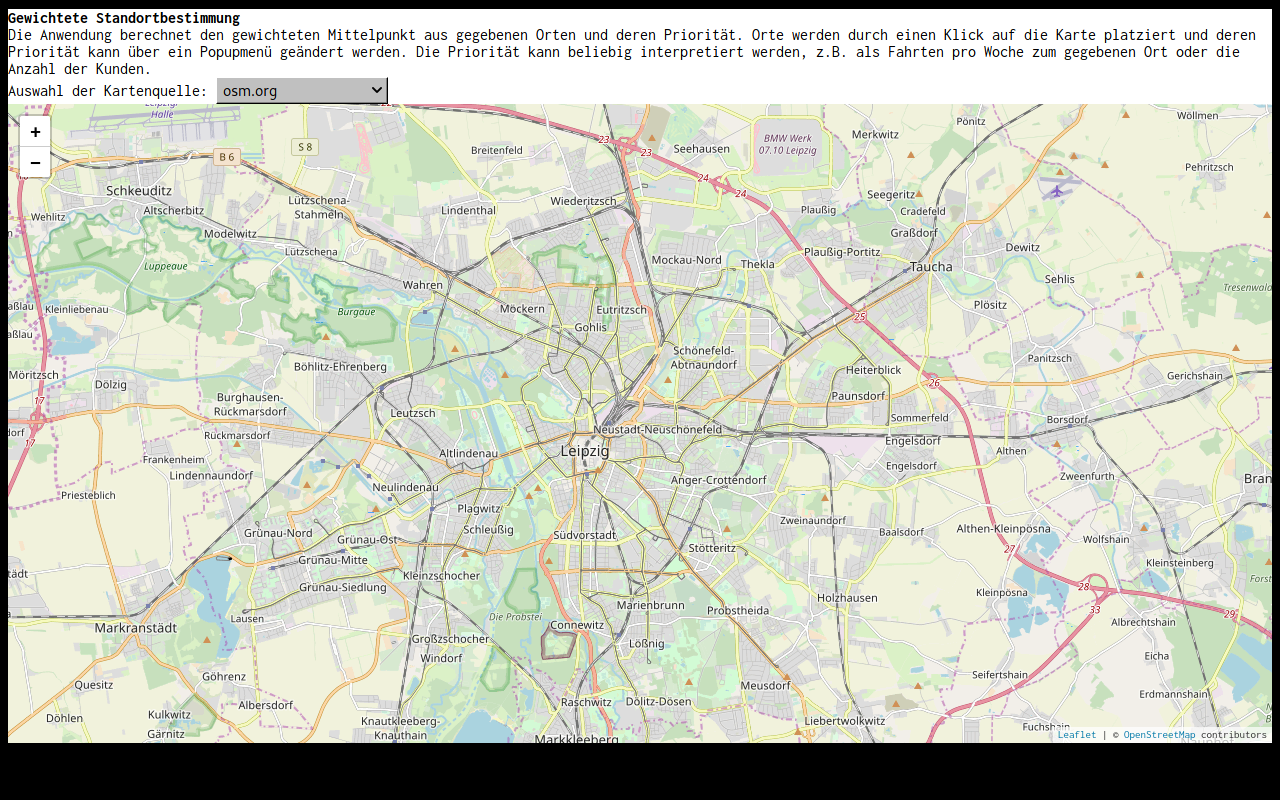
\includegraphics[height=6cm, width=10cm]{bell1_1.png}\\
Auf dieser Karte können nun Orte angeklickt werden, woraufhin ein Marker an der entsprechenden Position gesetzt wird. Auch wird direkt ein Mittelpunkt berechnet der sich aus den Standartwerten der Marker berechnen lässt.\\
\includegraphics[height=6cm, width=10cm]{bell2_1.png}\\\\\\\\
Um die Priorität eines Markers zu ändern muss man diesen anklicken und dort die Priorität im Eingabefeld ändern. Auch kann man in dem Popup einen Knopf zum Entfernen des Markers drücken, falls man ihn nicht mehr braucht.\\
\includegraphics[height=6cm, width=10cm]{bell3_1.png}\\
\chapter{Diskussion}
\section{Auswertung}
Die Anwendung ist vor allem für Personen/Diensleister geeignet, die keine besonderen Ansprüche an den Standort haben. Da die Anwendung Wohnvorstellungen, wie das Wohnen auf dem Land außer Acht lässt. Auch ist diese Anwendung nicht geeignet für Personen, die bloß zu einem Standort pendeln, da dieser dann als optimaler Standort angegeben wird und man für diese Erkenntnis nicht extra eine Anwendung braucht.
\section{Ausblick}
Momentan berechnet die Anwendung die Entfernungen nur per Luftlinie und lässt Straßen und natürliche Hindernisse, wie zum Beispiel Gewässer und Wälder, außer Acht.
Auch basiert die Berechnung bisher nur auf Linien in der Ebene, aber die Erde ist ein drei dimensionales Objekt und der Abstand zwischen zwei Punkten müsste durch einen Kreisbogen beschrieben werden.
Somit besteht noch viel Spielraum für die Erweiterung der Anwendung, zum Beispiel Integration von einem Wegfindealgorithmus, einer veränderten Distanzrechnung(beispielsweise über die gebrauchte Zeit, ...) .
Die Integration von Mietpreisen könnte auch bei der Entscheidung über den Standort helfen.
Auch die Speicherung der durch den Nutzer eingegebenen Daten in Cookies oder auf dem Server würde die Nutzerfreundlichkeit erhöhen. Oder man entwickelt eine Anwendung für Smartphones, die die Standortdaten über einen gewissen Zeitraum sammelt und diese Daten dann verarbeitet.
\bibliographystyle{unsrt}
\bibliography{bell}
\end{document}